\documentclass[10pt]{article}

\usepackage{fancyhdr}
\usepackage[includeheadfoot,left=1in, right=1in, top=0.5in, bottom=0.5in]{geometry}
\usepackage{lastpage}
\usepackage{extramarks}
\usepackage[usenames,dvipsnames]{color}
\usepackage{graphicx}
\usepackage{graphics}
\usepackage{listings}
\usepackage{courier}
\usepackage{float}
\usepackage{url}
\usepackage{subfigure}
\usepackage{varwidth}
\usepackage{caption}
\usepackage{multirow}
\usepackage[pdfborder={0 0 0}]{hyperref}
\usepackage[compact,small]{titlesec}
\usepackage{microtype}
\usepackage{verbatim}
\usepackage{booktabs}
\usepackage{indentfirst}
\usepackage{pgffor}
\usepackage[table]{xcolor}

\usepackage{amsmath}
%\usepackage[fleqn]{amsmath}

\rowcolors{2}{gray!25}{white}

\parskip = 0.5\baselineskip
\setlength{\belowcaptionskip}{-\baselineskip}

\captionsetup{font=scriptsize}
\captionsetup{labelfont=bf}

\pagestyle{fancy}
\rhead{Stack Attack}
\lhead{Network Security}
\rfoot{Page\ \thepage\ of \protect\pageref{LastPage}}
\cfoot{}
\renewcommand\headrulewidth{0.4pt}
\renewcommand\footrulewidth{0.4pt}

% make verbatim text small
\makeatletter
\g@addto@macro\@verbatim\tiny
\makeatother

\setlength\parindent{0pt} % Removes all indentation from paragraphs

\definecolor{sh_comment}{rgb}{0.12, 0.38, 0.18 } %adjusted, in Eclipse: {0.25, 0.42, 0.30 } = #3F6A4D
\definecolor{sh_keyword}{rgb}{0.37, 0.08, 0.25}  % #5F1441
\definecolor{sh_string}{rgb}{0.06, 0.10, 0.98} % #101AF9

\lstset{
    language=python,
    xleftmargin=.25in,
    xrightmargin=.25in,
    numbers=left,
    numberstyle=\tiny,
    frame=tb,
    showstringspaces=false,
    captionpos=b,
    stringstyle=\color{sh_string},
    keywordstyle = \color{sh_keyword}\bfseries,
    commentstyle=\color{sh_comment}\itshape,
    %basicstyle=\footnotesize\sffamily,
    basicstyle=\scriptsize\sffamily,
    %numbersep=-5pt,
    belowskip=\baselineskip,
    aboveskip=\baselineskip
}

\let\oldtabular\tabular
\renewcommand{\tabular}{\footnotesize\oldtabular}

\newcommand{\placementimage}[2]{
    \begin{figure}[H]
        \centering
        \includegraphics[width=\linewidth, height=4in, keepaspectratio]{#1}
        \caption{#2}
    \end{figure}
}

\newcommand{\specialcell}[2][c]{\textbf{\begin{tabular}[#1]{@{}c@{}}#2\end{tabular}}}

\title{
    %Cover page with student’s name, title of the report, date submitted and the
    %statement “Submitted as the Capstone Project for the Master of Engineering
    %Degree”
    \vspace{2in}
    \textmd{\textbf{CS6053 - Network Security}}\\
    \vspace{4in}
}
\author{\textbf{Stack Attack}}

\begin{document}
\maketitle
\newpage
\parskip = 0.2\baselineskip
\newpage
\tableofcontents
%\newpage
\listoffigures
\listoftables
%\lstlistoflistings
\parskip = 0.5\baselineskip
\newpage

\section{Maintaining Security}

In order to maintain a secure connection with the monitor we have implemented a
few different algorithms: Diffie-Hellman, Karn Symmetric Cyrptosystem, and the
Fiat-Shamir Algorithm.

\subsection{Diffie-Hellman}
In order to authenticate with the \texttt{Monitor} we first needed to implement
a shared secret key. We did this by implementing the Diffie-Hellman protocol. The
Diffie-Hellman key exchange works as shown below:
\begin{figure}[H]
    \centering
    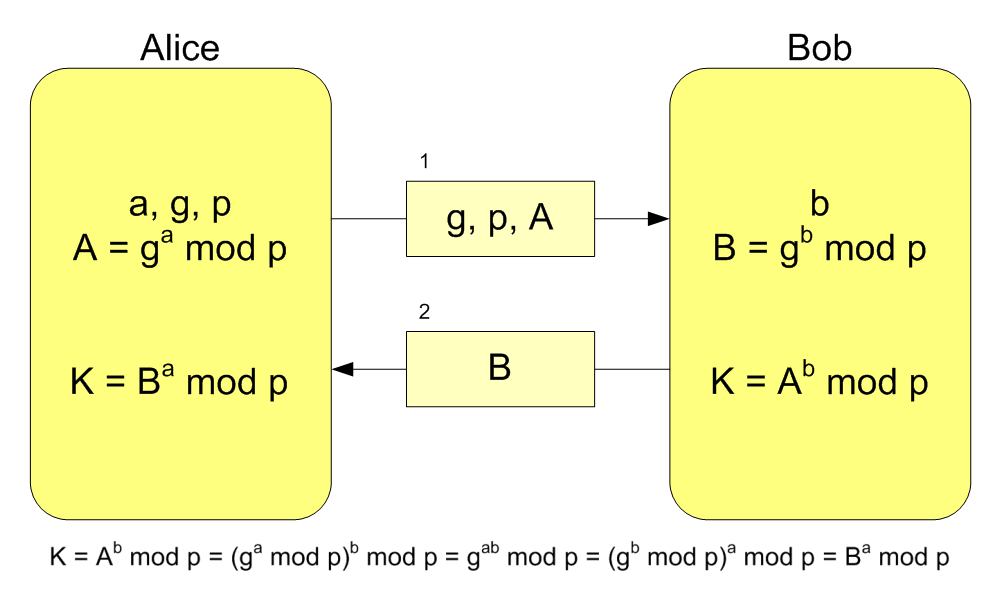
\includegraphics[width=0.4\linewidth]{./diffie_hellman.png}
    \caption{Diffie-Hellman Key Exchange}
\end{figure}
In the image above, we can see that \texttt{g,p} are just the generator and
the modulo prime number respectively. \texttt{A} is calculated using the
function, \texttt{K} (g$^{a}$ mod p); this is then sent over to \texttt{Bob}.
Note that \texttt{g,p}, and \texttt{A} are all seen by everyone. The trick here
is that \texttt{Alice} and \texttt{Bob} both generate there own secret key
locally (this key is never sent across a network). The way we can authenticate
can be shown in the example below:

\begin{align*}
    A &= g^{a} \thickspace mod \thickspace p,  \\
    B &= g^{b} \thickspace mod \thickspace p,  \\
    A &= 3^{15} \thickspace mod \thickspace 17 \equiv 6 \\
    B &= 3^{13} \thickspace mod \thickspace 17 \equiv 12 \\
\end{align*}
where a = 15 (Alice's secret key), g = 3, p = 17 and \\
where b = 13 (Bob's secret key),   g = 3, p = 17 \\

Therefore, \texttt{Bob} receives this value from \texttt{Alice} along with
\texttt{p} and \texttt{g}. Now \texttt{Bob} computes his result and sends
\texttt{12} to \texttt{Alice}. Now the heart of the trick lies here:
\texttt{Alice} will take Bob's key and use her private key to get the correct
message from \texttt{Bob} and \texttt{Bob} does the same with \texttt{Alice's}
key:

\begin{align*}
    A &= 12^{15} \thickspace mod \thickspace 17 \equiv 10 \\
    B &= 6^{13} \thickspace  mod \thickspace 17 \equiv 10
\end{align*}

The reason this works is because when you take an exponent to another exponent, these values get
multiplied:

\begin{align*}
    3^{13^{15}} \thickspace mod \thickspace 17 \equiv 3^{15^{13}} \thickspace mod \thickspace 17
\end{align*}

Therefore, even if Eve performed a man-in-the-middle attack, all Eve would have
is just the encrypted message and the prime and the generator number--making it
rather difficult to decrypt the message via brute-forcing due to the discrete
logarithm problem.

% encrypting with symmetric key
\subsection{Karn Symmetric Cryptosystem}
After implementing the Diffie-Hellman protocol we then needed to implement the
Karn encryption scheme. The Karn encryption scheme uses the Secure Hash
Algorithm (SHA-1) in order to generate the message digests. This algorithm uses
the shared keys generated by the Diffie-Hellman protocol. It initially splits
the bits of the shared secret key into two halves: a left and a right half. The
encryption algorithm works as described below \cite{karn}:
\begin{itemize}
    \item Add ``guard'' byte of value 42,
    \item During each block of plaintext, divide block of plaintext into
          left/right half,
    \item Find the message digest of the concatenation of the left plaintext
          half and the left key half,
    \item XOR the digest with the right plaintext half. (This produces the
          right ciphertext half),
    \item Find the message digest of the ciphertext right half concatenated
          with the key right half,
    \item XOR the digest with the plaintext left half.
\end{itemize}
Once this is complete we have both halves, allowing us to output both the left
and right half of the ciphertext.

In order to decrypt the message we needed to follow the steps shown below \cite{karn}:
\begin{itemize}
    \item Strip guard byte,
    \item For each ciphertext block, split the block into a left half and a
          right half,
    \item Find the message digest of the ciphertext right half concatenated
          with the key right half,
    \item XOR the result with the ciphertext left half to obtain the plaintext
          left half,
    \item Find the message digest of the plaintext left half and the key left
          half,
    \item XOR the result with the ciphertext right half to get the plaintext
          right half.
\end{itemize}

One interesting problem we came across is that the monitor is using a Java
BigInteger type to store its key and the BigInteger is signed so Java adds a
pad byte to maintain its signedness. This results in a key that is one byte
longer than we expect. Since we are using Python we have to manually add the
extra pad byte. This should really be fixed in the monitor
(\texttt{monitor/Cipher.java:87}) so that the pad byte is ignored.

\newpage
\subsection{Zero-Knowledge Proof}
A zero-knowledge proof is a proof that will prove a given statement
without giving out the ``answer.'' It only gives out the
``postulates/theorems'' to convince the server that the statement is true
without having the server learn anything about the given statement. One example
of a zero-knowledge proof is the Fiat-Shamir heuristic algorithm. A simple example
can be descibed below:

\texttt{Alice} (prover) will not need to have a shared key with \texttt{Bob}
(verifier); all Alice needs to do is convince \texttt{Bob} that this is truly
her without \texttt{Bob} having the key. \texttt{Alice} will prove the
knowledge of the secret to \texttt{Bob} in \texttt{t} executions. The
probability is found to be \texttt{2$^{-t}$}. Therefore, the more iterations
\texttt{Alice} tries to prove to \texttt{Bob}, the harder it is for an attacker
to ``impersonate'' \texttt{Alice/Bob}.

The protocol can be described below:
\begin{itemize}
    \item Initially, \texttt{A} will select two primes \texttt{p,q}, and multiply them together to generate the public key (n).
    \item \texttt{A} will then select \texttt{s} coprime to \texttt{n}, where $1 \leq s \leq$,
    \item \texttt{A} will then compute v:
        \begin{align*}
            v &\equiv s^{2} \thickspace mod \thickspace n
        \end{align*}
    \item \texttt{A} chooses random commitment \texttt{r}, $1 \leq \texttt{r} \leq \texttt{n-1}$
    \item \texttt{A} sends \texttt{B}:
        \begin{align*}
            x &\equiv r^{2} \thickspace mod \thickspace n
        \end{align*}
    \item \texttt{B} then sends \texttt{A} a random \texttt{e}, \{0,1\}
    \item \texttt{A} sends \texttt{B}:
        \begin{align*}
            y &\equiv r*s^{e} \thickspace mod \thickspace n
        \end{align*}
\end{itemize}
Once \texttt{A} has tried to prove to \texttt{B} that this is the correct user, \texttt{B} must verify.
The verification process is shown below:

\begin{itemize}
    \item \texttt{B} rejects if y = 0,
    \item \texttt{B} accepts if:
        \begin{align*}
            & y^{2} \equiv x*v^{e} \thickspace mod \thickspace n, \\
            & rejects \thickspace otherwise
        \end{align*}
\end{itemize}

We initially had a difficult time implementing this and ended up closely following
AJ Alts and Ryan Childs implementation \cite{aj} from a few years ago.

\newpage
\section{Attacking Accounts}

We entered this competition from a purely defensive standpoint, mostly due to
the fact that we didn't have our code fully working until a few days before the
competition. When the competition began we waited for a while to see what the
activity of the other players would be. After seeing basically no activity for
almost an hour we decided to just start our script that would transfer funds
between our accounts. As other players connected we manually recorded their
cookies (later wrote a script to harvest them) in anticipation of being able to
use them later. It wasn't long before somehow our password was changed. At the
time this was really baffling because we had never sent our password to the
monitor and you need the old password to create a new one. As we later found
out the team that got root on gauss had full control of the monitor. At this
point we were unable to do much. We added the functionality to parse the logs
for our latest cookie and password in an attempt to recover our accounts. This
was fruitless, however, being that every time the other team logged in with our
account they immediately changed the password again causing the cookie to
change.  We left our script running anyway in the hopes that maybe their
strategy would change and we would be able to grab the new password to our
account. Needless to say we were never able to recover our account and the
points we had accrued early in the competition were taken back by the monitor
over time as our server was not able to respond to the alive requests.

\vfill
\begin{figure}[H]
    \centering
    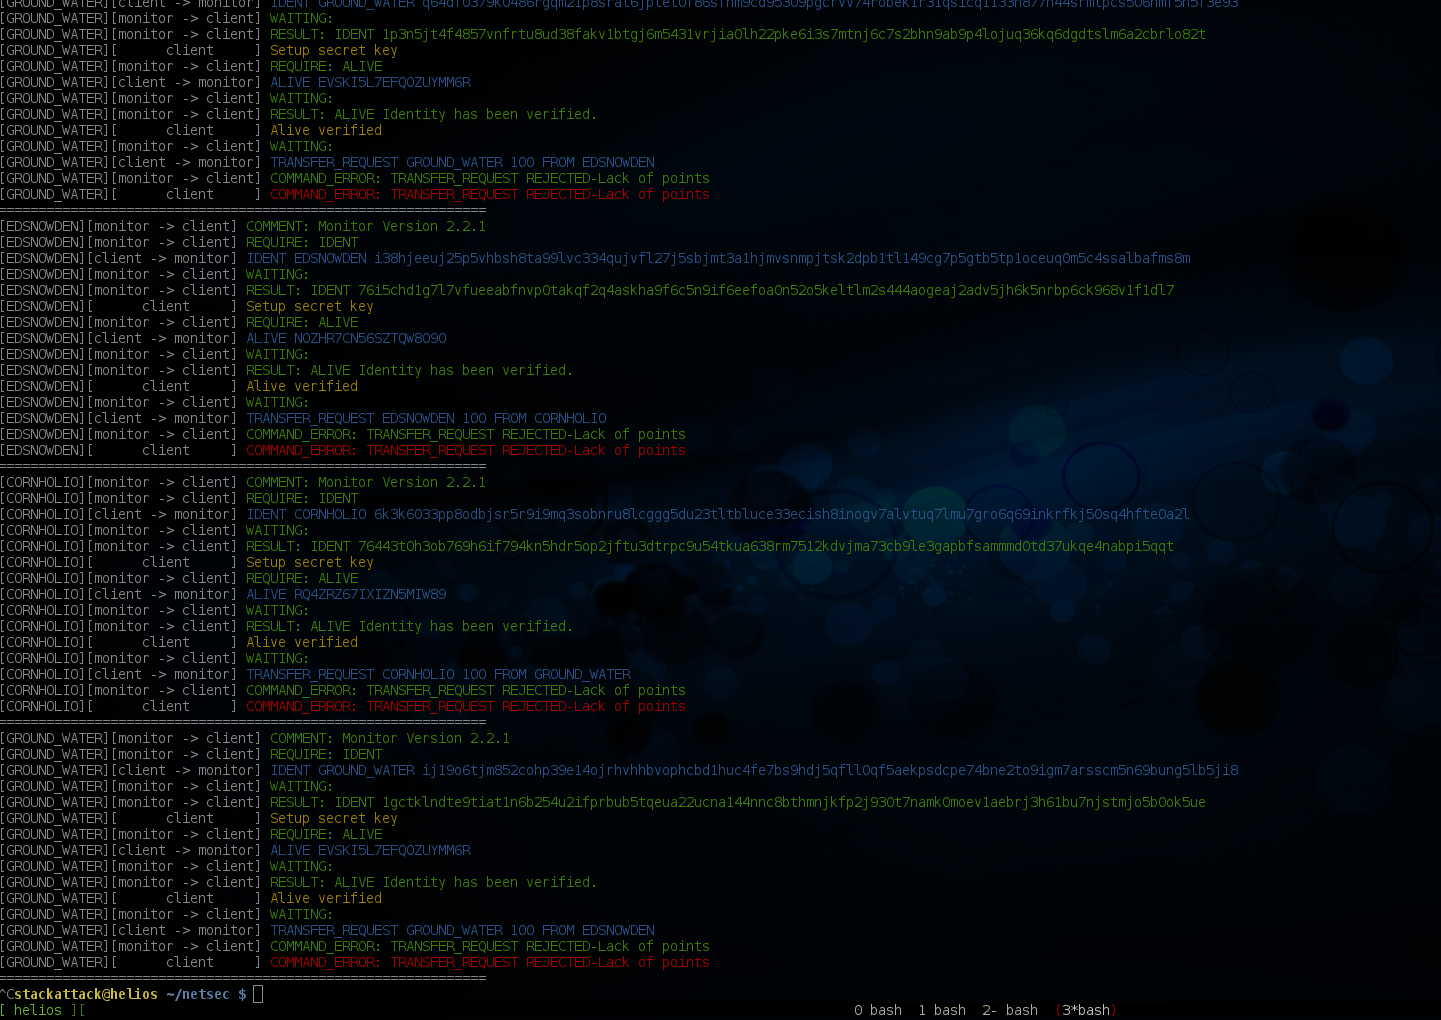
\includegraphics[width=\linewidth]{./log.png}
    \caption{Screenshot of script transferring points between our three accounts}
\end{figure}
\vfill

\newpage
\section{Appendix}
    \subsection{Python Code}
    \lstinputlisting[caption=\textbf{Client}]{../client.py}
    \lstinputlisting[caption=\textbf{Server}]{../server.py}
    \lstinputlisting[caption=\textbf{Diffie Hellman}]{../diffie_hellman.py}
    \lstinputlisting[caption=\textbf{Karn}]{../karn.py}
    \lstinputlisting[caption=\textbf{Fiat-Shamir - Zero Knowledge Proof}]{../fiat.py}
    \lstinputlisting[caption=\textbf{Printer}]{../printer.py}
    \lstinputlisting[caption=\textbf{Base 32}]{../base32.py}
    \lstinputlisting[caption=\textbf{Configuration File}]{../config.py}

\newpage
\begin{thebibliography}{9}
    \bibitem{zero} \url{http://www.cs.princeton.edu/courses/archive/fall07/cos433/lec15.pdf}
    \bibitem{aj} \url{https://github.com/ajalt/PWNmlete-2011/blob/master/fiat_shamir.py}
    \bibitem{karn} \url{http://gauss.ececs.uc.edu/Courses/c6053/homework/assgn3.html}
\end{thebibliography}

\end{document}
